\chapter{Aspects techniques}

	\section{Librairie piecesPuzzle}

        Pour la conception de ce projet, une librairie a été créer, réferencant ainsi toutes les pièces possibles. Cette librairie comporte 4 pièces différentes. Ces quatres pièces ont toutes une grille créer a partie de la rotation défini. Cette grille et cette rotation est créer à l'aide de la méthode \textit{createGrid()} qui prend en paramètre un numéro qui correspond a la rotation dans le sens horaire. Cette méthode change la largeur/longueur de la pièce, en fonction de celle données de la pièce de départ, permettant ainsi la création d'une nouvelle grille en prenant en compte la rotation.
        Chaque pièce a une grille composé de valeur boolean, permettant ainsi de créer la pièce voulu (valeur "true" pour indiquer que la case est pleine), en fonction de sa rotation, largeur, longeur. Elle est aussi composé de coordonnées, permettant, en fonction du jeu, de pouvoir situé la pièce dans le plateau.

    \section{Modèle : Le plateau}

        La librairie piecesPuzzle est utiliser par notre modèle. PlateauPuzzle permet de créer un plateau ainsi que d'utiliser les pièces pour les ajouter, supprimer...
        Pour la création de notre plateau, nous avons utiliser une HashMap de coordonnées (ArrayList de Integer) en clé et d'une pièce, s'il y en a une, ou "null" en valeur. Cela permet donc d'avoir une lisibilité absolut sur le plateau, ainsi que sur les différentes pièces présentes, sans être obliger d'avoir une hashmap trié.
        La HashMap est directement créer dès l'appel à cette classe.

        Le plateau peut donc créer, placer, supprimer, déplacer, tourner la pièce sur le plateau. Pour la plupart des différentes méthodes, un appel de la méthode \textit{validePlacement()\label{txt:validePlacement}} est nécessaires afin de savoir si la pièce, reçu par la méthode, peut être placer dans le HashMap. Pour cela, dès que la valeur de la grille parcouru est de boolean \textit{true}, elle regarde si la valeurs de la clé coordonnées du HashMap (en fonction des coordonnées reçu par la méthode). Cela permet donc de pouvoir placer des pièces cote a cote, en ne placant que les case "true" de la pièce dans la HashMap.
        Les pièces ont donc des cases "true" et "false" en fonction de comment elles sont créer. Nous avons choisit une case de référence afin d'avoir les coordonnées de la pièce s'il faut, par exemple, la déplacer ou la faire tourner, ou encore, si on sauvegarde la partie. Cette case de référence, nous l'avons choisis en haut à gauche de la pièce.
        Sauf que cela posait problème si le joueur voulait posé la pièce a l'endroit où il a cliquer/indiquer les coordonnées (voir image\ref{img:prblmPlacement}). En effet, la case est toujours en haut a gauche, même si cette case est en false.

        \begin{table}[h]\label{img:prblmPlacement}
            \centering
            \begin{tabular}{cc}
                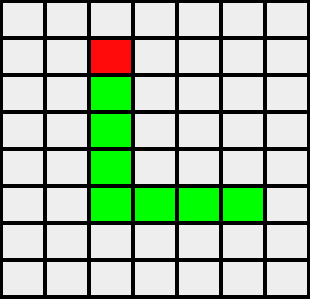
\includegraphics[width=0.20\textwidth, keepaspectratio]{img/pieceLrot0.png} & 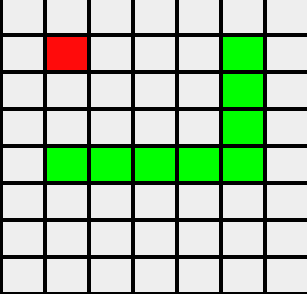
\includegraphics[width=0.20\textwidth, keepaspectratio]{img/pieceLrot3.png}\\
            \end{tabular}
            \begin{tabular}{c}
                Légende:\\
                Rouge: coordonnées où le joueur veut placer la pièce, et indique aussi la case de référence\\
                Vert: pièce L en rotation 0 (img 1) et rotation 3 (img 2)
            \end{tabular}
       \end{table}

       Pour régler ce problème, nous avons rajouter un changement de coordonnées, dès que le joueur indiquait, par un clique ou par indication de coordonnées en console, la case où il voulait placer la pièce. Tant que les coordonnées Y de la grille de la pièce était false, les coordonnées (\textit{coo}) en position Y était diminuer de -1, permettant ainsi de placer la grille de la pièce a partir des coordonnées indiqué -1, si la case était "true" .

       \begin{algorithm}[H]\label{alg:whilePlacementPiece}
		         \caption{finished():boolean}
                 $posY \leftarrow 0$\;
                 $xx \leftarrow 0$\;
                 $yy \leftarrow 0$\;
                 \While{$!piece.getGrid()[xx][yy+posY]$}{
                    $coo.set(1, coo.get(1)-1)$\;
                    $posY \leftarrow posY+1$\;
				}
				\Return true
			\end{algorithm}

        Cela permet de changer la "case", donc les coordonnées indiquer par le joueur, jusqu'à ce que la valeur des coordonnées de la grille de la pièce est égal a "true".

        \begin{center}
            \begin{tabular}{|m{4.5cm}|m{4.5cm}|m{4.5cm}|}
                \hline
                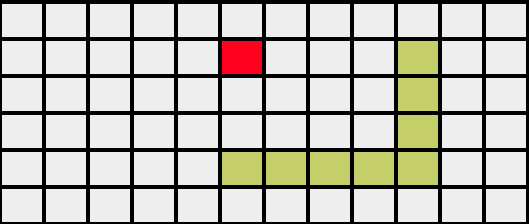
\includegraphics[width=0.20\textwidth, keepaspectratio]{img/pieceLCliqueFantome.png} & 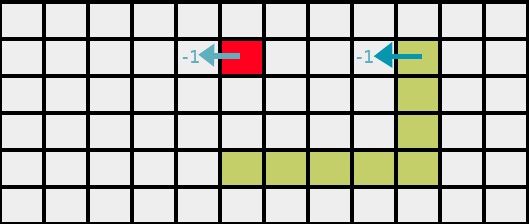
\includegraphics[width=0.20\textwidth, keepaspectratio]{img/pieceLCliqueFantome-1.png} & 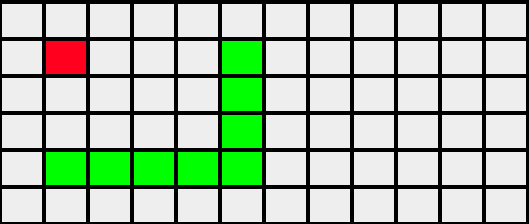
\includegraphics[width=0.20\textwidth, keepaspectratio]{img/pieceLCliqueMis.png}\\
                \hline
                {\small Pris en compte des coordonnées} & {\small Boucle while} & {\small Application de l'ajout ou déplacement de la pièce}\\
                \hline
            \end{tabular}
        \end{center}

            \begin{tabular}{|m{13.5cm}|}
                \hline
                {\small Légende:}\\
                {\small Rouge: Case de référence et variable "coo" qui, sur l'image 1, sont les coordonnées renseigner par le joueur (modifier par la suite dans la while)}\\
                {\small Flèche: coo modifier dans la while}\\
                {\small Vert/jaune: Pièce "fantome" où la pièce devrait être normalment sans cette while}\\
                \hline
            \end{tabular}

            Cela permet de changer la "case", donc les coordonnées indiquer par le joueur, jusqu'à ce que la valeur des coordonnées de la grille de la pièce est égal a "true".\\
            Pour cela, pendant que la valeurs des coordonnées Y de la variable \textit{coo} diminuent, le parcours de la grille se fait jusqu'à ce que elle rencontre la case plus en haut a gauche possible de la pièce. Donc elle ajoute +1 a la variable \textit{posY}.\\
                \\

                \begin{table}[h]\label{img:prblmPlacementPiece}
                    \begin{tabular}{c}
                        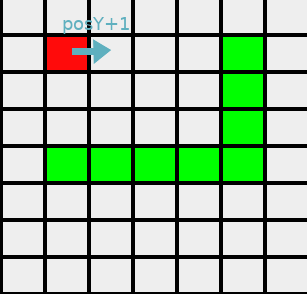
\includegraphics[width=0.20\textwidth, keepaspectratio]{img/pieceLposY.png}
                    \end{tabular}
                    \begin{tabular}{l}
                        {\small Légende:}\\
                        {\small Rouge: Case de référence}\\
                        {\small Flèche: vérification de la prochaine case si sa valeur est "true"}\\
                        {\small Vert: pièce L rotation 3}\\
                    \end{tabular}
               \end{table}


      \section{Controleur}

        Le controleur est séparrés en plusieurs classes:
        \begin{description}
            \item[classe \textit{PlayMenu}:]{Permet de choisir entre la vue console et la vue graphique.}
            \item[classe \textit{Play}:]{Fait appel aux méthodes du modèle,et appels les méthodes de "choix" en fonction de la vue/joueur actuel.}
            \item[classe \textit{InterfacePlay}:]{Méthodes communes aux choix des joueur: ia ou joueur.}
            \item[classe \textit{PlayJoueur}:]{Méthodes de choix pour joueur Console, grâce aux Scanner.}
            \item[classe \textit{PlayIa}:]{Méthodes de choix pour ia.}
            \item[enum \textit{EnumAction}:]{Enumère les actions possibles en jeu.}
		\end{description}


        \begin{figure}[H]
			\centering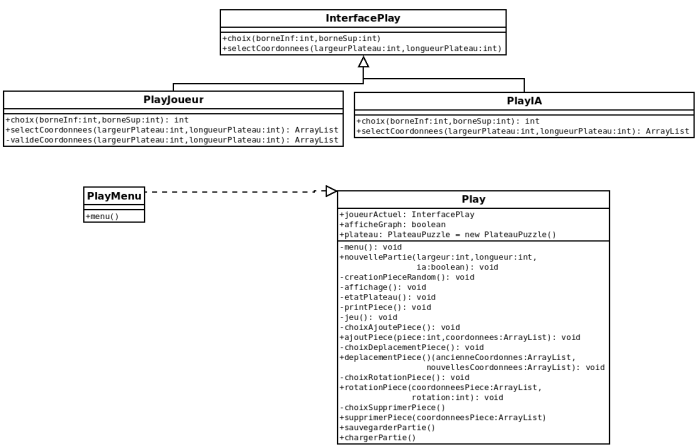
\includegraphics[width=0.64\textwidth, keepaspectratio]{img/diaControleur.png}
			\caption{Controleur}
			\label{fig:diaControleur}
		\end{figure}

        Cette séparations permet simplifier et séparer les choix de jeu. Cela évite la redondance de code.

        \subsection{Play}

        En vue console, les choix se font grâce à la variable \textit{joueurActuel} qui est une instance de \textit{InterfacePlay}. Cela permet, en fonction du choix du joueur (option ia ou non), d'appeller les même méthodes de choix, permettant ensuite d'appeler les méthodes communes a toutes les vues pour accomplir l'action prévu (placer, déplacer...). Tout cela est controler par la méthode \textit{jeu()}.

        \begin{figure}[H]
			\centering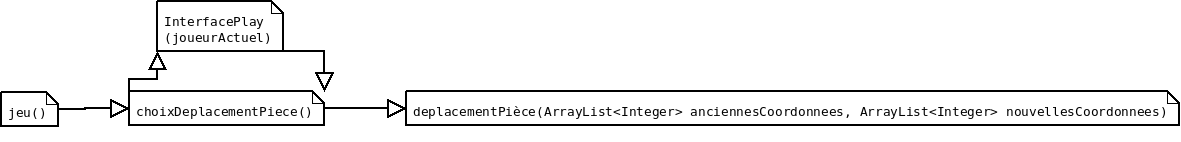
\includegraphics[width=0.64\textwidth, keepaspectratio]{img/graphJoueurChoix.png}
			\caption{Explication choix en fonction du joueur - vue console}
			\label{fig:graphJoueurChoix}
		\end{figure}

        En vue graphique, les choix se font grâce à des actions sur des cases/boutons, détecter par des Observeur/Observable voir...partie graph

        \subsubsection{Joueur Ia}\label{subsub:jeuIa}
        Une méthode \textit{jeuIa()} est appeler dès que le joueur choisis de regarder l'ia joué une partie chargé ou une nouvelle partie (en vue graphique ou console). Cette option permet donc de savoir la meilleurs composition de jeu.
        Cette méthode permet de lancer des \textit{fourmis} (joueur ia qui joue une partie avec des choix random et guidées) afin de faire un certain nombre de partie. Le meilleurs score et le meilleurs plateau est enregistrer. Cela permet donc d'avoir plusieurs possibilités aléatoires, et d'essayer de trouver la meilleurs composition possible. Cela évite donc de n'avoir qu'une possibilité qui regarde jusqu'à une certaine profondeur.

        La fourmis appel donc la méthode \textit{jeu()}, commune si le joueur actuel est le joueur en vue console. Cette méthode permet de choisir l'action que le joueur va effectuer. C'est un choix, donc cette mathode appel l'attribut \textit{joueurActuel}, permetant de faire un choix random pour  l'ia. Pour éviter d'avoir un simple choix aléatoire où toutes les actions ont le même niveau de piorité, une liste d'actions a été créer avec plusieurs même actions à l'interieur, permettant de signifier qu'une action pour "avancer" (placer et déplacer) dans le jeu est plus important que de "rester sur place" (rotation dans le plateau et rotation des pièces a jouer) et est plus important qu'une action qui "recule" l'avancement du jeu (supprimer une pièce). Une fois l'action choisis, d'autres méthodes de choix sont appelés en fonction du choix de l'action.

        Pour les actions pour "avancer" dans le jeu, les choix ne sont pas de simple random. En effet, si la fourmis a choisi l'action de PLACER ou DEPLACER une pièce, la méthode \textit{choixDeplacement()} ou \textit{choixAjout()} est appelé. Ces deux méthodes prenent en compte la largeur, la longueur et le plateau.
        Pour \textit{choixDeplacement()}, l'ia choisis d'abord une pièce au hasard sur le plateau, grâce à la méthode selectPiece() (méthode commune de l'InterfacePLay) qui sélectionne une pièce dans la liste des pièces placer. Les coordonnées récupéré sont les coordonnées de la case de référence de la pièce (cf: voir \ref{img:prblmPlacement}). Une boucle while, presque similaire  à ici\ref{alg:whilePlacementPiece}, est donc nécessaire pour avoir les coordonnées qui aurait pu être cliquer ou indiquer par un véritable joueur. Une fois les coordonnées obtenus, la pièce est supprimer afin d'exercer une simulation de possibilité sans avoir une pièce sur ces cases dans le plateau.
        A partir de la, \textit{choixDeplacement()} exerce comme \textit{choixAjout()}. Elles créer une copie du plateau actuel, puis parcours tout le plateau à l'aide des coordonnées placé en clé du HashMap. Si la coordonnée est vide et au moins une pièce est situé à 1 ou 2 cases autour de celle ci, alors un test de placement est fait (grâce à la méthode \textit{validePlacement()}\ref{txt:validePlacement}). Si ce test est réussi, un deuxième test est necessaire: faire un ajout de la pièce aux coordonnées et calculer le score grâce aux méthodes dans la classe \textit{PlateauPuzzle}). Si le score est supérieur au score du test précédent, une sauvearde du score et des coordonnées est faites. Sinon, cela passe au test pour les coordonnées suivantes.
        Le \textit{validePlacement()} est déjà appeller dans la méthode d'ajout ou de déplacement, mais cela diminue de temps d'execution en vérifiant le placement avant d'appeler la méthode d'ajout qui vérifie le placement et qui place si c'est possible.

        Pour les autres actions (Rotation, Supprimer), le choix est défini en aléatoires.

        Une fois que toutes les fourmis ont finit leurs parties, \textit{afficheIa()} affiche le plateau ayant obtenus le meilleurs score. L'affichage déplace d'abord les pièces déjà placer sur le plateau initiale(si c'est une partie charger), puis place ensuite les pièces a jouer en fonction du plateau obtenus par les fourmis. Pour cela, elle utilise les méthodes communes pour effectuer des actions.

        \subsubsection{joueur Graphique}
        Si la vue graphique est choisis, une InterfaceGraphique, une MouseClicker ainsi qu'un ActionGraphique est créer a partir du constructeur de la classe \textit{Play()}, permettant ainsi d'afficher la Vue. Ensuite, la méthode \textit{menuGraph()} est appeler, permettant d'appeler \textit{jeuIa()} ou \textit{jeuVue} en fonction de ce que veux le joueur. Le choix se fait grâce aux différents boutons. Le joueur peut donc sélectionné la taille de son plateau (via le bouton ligne et colonne qui vont de 5 à 20), il peut également charger une partie, afficher le tableau des scores ou encore les règles du jeu. Le fonctionnement des boutons sont assez simple. Le controleur attend que ActionGraphique le notifie, pemrettant ainsi de récuperer le choix du joueur (via la méthode \textit{getChoix()}) et ordonne ainsi à la vue ce qu'elle doit faire (afficher la grille, les scores, demander au joueur de selectionné une pièce,...).

        \begin{figure}[H]\label{img:joueurGraphqiue}
            \centering
            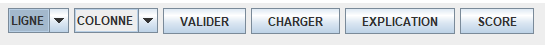
\includegraphics[scale=0.8]{img/menu.png}
            \caption{Bouton du menu principal}
        \end{figure}


    \section{Vue}
        La vue est composé de 3 classes :
        \begin{description}
            \item[classe \textit{InterfaceGraphique}:]{Construit et affiche la vue graphique }
            \item[classe \textit{ActionGraphique}:]{Gère les interactions entre le joueur et la vue}
            \item[classe \textit{MouseClicker}:]{Permet de récupéré les clique souris du joueur sur la vue}
		\end{description}

		\subsection{InterfaceGraphique}
		L'interface Graphique est composé de nombreuses méthodes pour afficher la vue. La méthode principale est \textit{buildContentPane()}.Elle permet à la fenêtre, dans un premier temps, d'afficher le menu principale lorsqu'elle n'a pas de modèle. Ce menu est composé de divers bouton (cf: voir \ref{img:joueurGraphqiue}). Et quand nous avons un modèle, on affiche la grille en parcourant le plateau en vérifiant la présence de pièce. Cette grille est une grande fenêtre de couleur noir composé de plusieurs petites fenêtre grise espacé entre-elles, donnant cette impression de grille. On oublie pas d'ajouter à cela les pièces à placer, les boutons de jeu et les rotations des pièces, nous obtenons ceci \ref{img:plateau}. Cette class permet aussi l'affichage des scores, des explications de jeu, des aides, du formulaire pour rentrer son pseudo et des fenêtre de choix.

        \begin{figure}[H]
            \centering
            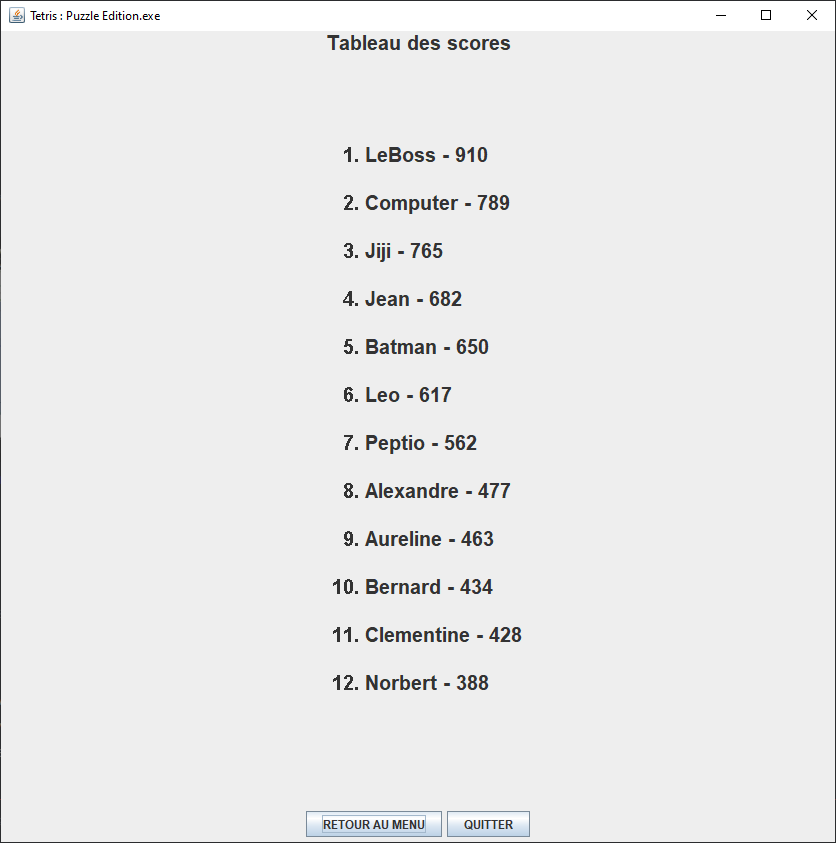
\includegraphics[scale=0.5]{img/score.png}
            \caption{Tableau des scores}
        \end{figure}

        \subsection{ActionGraphique et MouseClicke}
        Ces 2 méthodes sont liés car MouseClicker est utilisé quand les méthodes d'interaction d'ActionGraphique sont appelés. La tache d'ActionGraphique est d'attribuer un rôle à chaque bouton et de gérer l'ordre des évènements quand un joueur veut réaliser une action. Par exemple, le bouton "PLACER" va appelé la méthode \textit{actionBouton()} pour vérifier si aucune autre action est en cours. Si aucune action est en cours, on appelle la méthode \textit{placementPieceVue()} qui va demander au joueur de sélectionner une pièce. Il va attendre que MouseClicker lui envoie la pièce sélectionner pour ensuite demander au joueur de choisir sa rotation et son emplacement. Il va de nouveau attendre que MouseClicker lui envoie la case sélectionné pour pouvoir demander au contrôleur de placer la pièce dans la rotation souhaité via les méthodes vu précédemment. Pendant les 2 périodes où ActionGraphique attend, on vérifie si le joueur n'a pas décidé d'annuler son action, sinon on coupe l'attente est demande à la vue d'afficher son état initiale. Ce processus est semblable pour les méthodes \textit{deplacementPieceVue()} et \textit{supprimerPieceVue()}. Cette class gère aussi les listener des pièces et des case de la grille, pour que le joueur ne fasse pas de mauvaise sélection.
